\chapter{Introduzione}
Le api recano importanti benefici e servizi ecologici per la società. Con l’impollinazione le api svolgono una funzione strategica per la conservazione della flora, contribuendo al miglioramento ed al mantenimento della biodiversità.\newline 
In botanica, l’impollinazione è quel processo che consiste nel trasporto dei pollini dalla parte maschile e quella femminile dell’apparato riproduttivo delle piante. Grazie ad agenti atmosferici e sopratutto al lavoro incessante degli insetti impollinatori, soprattutto le api, il polline viene trasportato da una pianta all’altra rendendo possibile la fecondazione di un’essenza vegetale della stessa specie e la conseguente produzione di semi e frutti. Una diminuzione delle api può quindi rappresentare una importante minaccia per gli ecosistemi naturali in cui esse vivono. L’agricoltura, d’altro canto, ha un enorme interesse a mantenere le api quali efficaci agenti impollinatori. La Food and Agriculture Organization - FAO ha informato la comunità internazionale dell’allarmante riduzione a livello mondiale di insetti impollinatori, tra cui Apis mellifera, le api da miele. Circa l’84\% delle specie di piante e l’80\% della produzione alimentare in Europa dipendono in larga misura dall’impollinazione ad opera delle api ed altri insetti pronubi \cite{bellucciapi}. Pertanto, il valore economico del servizio di impollinazione offerto dalle api risulta fino a dieci volte maggiore rispetto al valore del miele prodotto.\newline 
Da un rapporto dell’Unione Internazionale per la Conservazione della Natura (LUCN) risulta che il 10\% delle specie selvatiche di api (apis mellifera) sarebbe in via di estinzione e un altro 5\% sarebbe a rischio. Una delle principali cause sono i pesticidi, i quali influenzano l’apprendimento, la capacità riproduttiva, i comportamenti sociali di questi insetti e l'orientamento. \newline
La mortalità delle api (Apis mellifera) è un fenomeno che si acuisce soprattutto in primavera e che rischia di compromettere la fondamentale funzione ecologica di questi insetti impollinatori per l’intero ecosistema.\newline
Un’indagine di campo del Centro di referenza nazionale per l’apicoltura dell’Istituto Zooprofilattico Sperimentale delle Venezie nell’ambito di alcune morie riscontrate ha rilevato la presenza, in campioni di api morte, di residui di pesticidi e di alcuni virus delle api. Le infezioni virali potrebbero peggiorare l’impatto già negativo dei pesticidi sulla salute delle api, mettendo ulteriormente in pericolo la sopravvivenza delle colonie.\newline
Lo studio è stato effettuato su 94 campioni, provenienti dal Nord-est dell’Italia e raccolti durante la primavera 2014, prendendo in considerazione 150 principi attivi e 3 virus delle api. Lo studio è pubblicato su Journal of Apicultural Research. I ricercatori hanno riscontrato la presenza di almeno un principio attivo nel 72,2\% dei campioni (api morte). Gli insetticidi sono i più abbondanti (59,4\%), principalmente quelli appartenenti alla classe dei neonicotinoidi (41,8\%), seguiti da fungicidi (40,6\%) e acaricidi (24,1\%). Gli insetticidi più frequentemente rilevati sono rappresentati da imidacloprid, chlorpyrifos, tau-fluvalinate e cyprodinil.\newline
La presenza di una possibile relazione tra la mortalità primaverile delle api e l’impiego di trattamenti antiparassitari in agricoltura potrebbe contribuire a comprendere meglio fenomeni complessi come la moria delle api e lo spopolamento degli alveari, che negli ultimi dieci anni hanno colpito questo settore\cite{martinello2017spring}.\newline
Lo scopo della presente tesi è quello di illustrare la progettazione di un software che visualizza come le molecole di specifici pesticidi si dispongono, in maniera spaziale, quando sono legate ai recettori delle api, questo processo viene definito \textbf{docking molecolare}, e successivamente il software estrae i legami che si vengono a formare.

\begin{figure}[H]
    \centering
    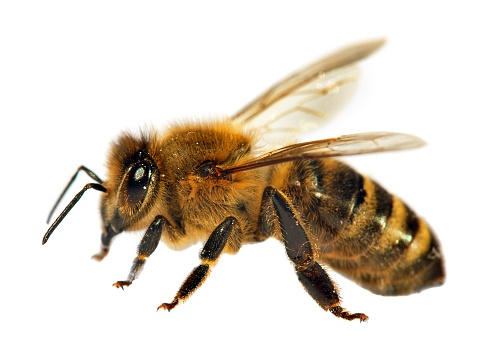
\includegraphics{immagini/apisMellifera.png}
    \caption{Esemplare adulto di Apis Mellifera}
    \label{fig:Apis Mellifera}
\end{figure}

\section{Docking Molecolare}
Il docking molecolare è una tecnica computazionale che mira a determinare le migliori conformazioni adottate da una molecola per legarsi ad un’altra al fine di formare un complesso stabile. Il docking molecolare viene fondamentalmente utilizzato per la valutazione delle interazioni ligando-target. A partire quindi da un ligando e dalla struttura nota del suo target, il docking molecolare permette di generare una serie di conformazioni possibili del ligando stesso localizzato all’interno del sito attivo della proteina. Esse sono denominate \textit{“binding poses”}e sono valutate da particolari funzioni chiamate \textit{“scoring functions”}, che creano quindi un vero e proprio ranking. Le \textit{migliori poses} rappresentano quella che viene identificata come la miglior soluzione proposta dall’algoritmo per l’interazione tra il ligando e il target\cite{meng2011molecular}.\newline
Gli algoritmi di docking sono formati da due componenti fondamentali: l’algoritmo di ricerca (o \textit{“search algorithm”}) e la \textit{“scoring function”}. Il primo si occupa di generare un insieme di
12 conformazioni del ligando all’interno del sito designato del target, mentre la seconda valuta le \textit{poses}
generate, assegnando a ciascuna di esse un punteggio (detto \textit{“score”}) in base a parametri di tipo geometrico ed energetico. Le migliori conformazioni in uscita da questa valutazione sono passate nuovamente all’algoritmo di ricerca, che andrà a creare una nuova generazione di conformazioni partendo dalle migliori soluzioni della run precedente. Il funzionamento iterativo del \textit{search algorithm} e della \textit{scoring function} permettono di ottenere, alla fine di un determinato numero di cicli, un insieme di \textit{poses} che vengono fornite come output all’utente e che sono ritenute essere le migliori soluzioni per il \textit{binding} delle molecole in esame da parte del programma di docking utilizzato.\newline
In generale, il docking molecolare è eseguibile in tre differenti condizioni, che si differenziano l’una dall’altra per i gradi di libertà tenuti in considerazione dall’algoritmo durante il calcolo: 

\begin{itemize}
    \item docking a corpo rigido, che approssima sia il ligando che la proteina come strutture rigide
    \item docking semi-flessibile, che considera il target come rigido, tendendo però in considerazione i gradi di libertà conformazionale del ligando
    \item docking flessibile, in cui vengono considerati i gradi di libertà sia del ligando che dei residui del target nel sito attivo.
\end{itemize}

Intuitivamente, passando da un approccio a corpo rigido fino ad uno flessibile, la complessità di calcolo aumenta, e, proporzionalmente, anche il tempo di esecuzione.\newline
Ad oggi sono disponibili diversi protocolli di docking, e ognuno sfrutta una particolare coppia algoritmo di \textit{ricerca-scoring function}.\newline
Il docking molecolare consiste in tre obiettivi principali collegati tra loro: predizione della posa, screening virtuale e stima dell'affinità di legame. Una metodologia di docking di successo deve essere in grado di prevedere correttamente la posa nativa del ligando all'interno del sito di legame del recettore (cioè di trovare la geometria sperimentale del ligando entro un certo limite di tolleranza) e le interazioni fisico-chimiche molecolari associate. Inoltre, quando si analizzano librerie di composti di grandi dimensioni, il metodo deve essere in grado di distinguere con successo le molecole che si legano da quelle che non si legano e di classificare correttamente questi ligandi tra i migliori composti del database. Un algoritmo di ricerca e una funzione di score energetico sono gli strumenti di base di una metodologia di docking per generare e valutare le conformazioni dei ligandi. La capacità di gestire con successo la flessibilità molecolare intrinseca di un sistema e di descrivere correttamente l'energia delle interazioni recettore-ligando è cruciale per lo sviluppo di metodologie di docking predittivo che sono utili negli studi prospettici di progettazione di farmaci\cite{guedes2014receptor}.

\begin{figure}[H]
    \centering
    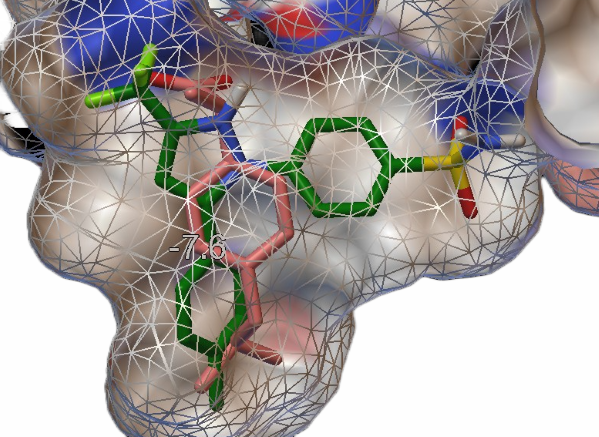
\includegraphics[scale=0.5]{immagini/dockingMolecolare.png}
    \caption{Rappresentazione dei due ligandi ibuprofene a sinistra e celecoxib a destra che hanno effettuato il docking con un enzima di COX2}
    \label{fig:Docking Molecolare}
\end{figure}

\section{Simulazione}
La simulazione di un processo di docking è un processo molto più che complicato. In tale approccio, la proteina e il ligando sono separati fisicamente da una certa distanza, e il ligando trova la sua posizione nel sito attivo della proteina dopo aver compiuto diversi movimenti nello spazio. Tali movimenti includono rotazioni, traslazioni e torsione di
alcuni angoli di rotazione degli atomi. Ognuno di questi movimenti ha un determinato costo energetico nel sistema, quindi dopo ogni mossa viene ricalcolata l'energia totale del sistema. Questo approccio modellizza molto precisamente quello che accade nella realtà. Di contro, il costo richiesto in termini di tempo e prestazioni è molto elevato.
    
\section{Software per il docking molecolare}
I programmi di docking molecolare eseguono un algoritmo di ricerca in cui la conformazione del ligando viene valutata ricorsivamente fino a raggiungere la convergenza all'energia minima. Infine, una funzione di punteggio di affinità, $\Delta$G (Energia potenziale totale in kcal/mol), viene impiegata per classificare le pose candidate come la somma delle energie elettrostatiche e di van der Waals. Le forze trainanti per queste specifiche interazioni nei sistemi biologici mirano alla complementarità tra la forma e l'elettrostatica delle superfici del sito di legame e del ligando o del substrato. \newline
Negli ultimi vent'anni, sono stati sviluppati più di 60 diversi strumenti e programmi di docking sia per uso accademico e commerciali, come DOCK (Venkatachalam et al. 2003) AutoDock (Österberg et al. 2002), FlexX (Rarey et al. 1996), Surflex (Jain 2003), GOLD (Jones et al. 1997), ICM (Schapira et al. 2003), Glide (Friesner et al. 2004), Cdocker, LigandFit (Venkatachalam et al. 2003), MCDock, FRED (McGann et al. 2003), MOE-Dock (Corbeil et al. 2012), LeDock (Zhao e Caflisch 2013), AutoDock Vina (Trott e Olson 2010), rDock (Ruiz-Carmona et al. 2014), UCSF Dock (Allen et al. 2015) e molti altri. \newline 
Tra questi programmi, AutoDock Vina, GOLD e MOE-Dock hanno predetto le pose migliori con gli score migliori. AutoDock e LeDock sono stati in grado di identificare i corretti legami dei ligandi nelle pose. Sia Glide (XP) che AutoDock hanno previsto le pose con un'accuratezza del 90,0\% (Wang et al. 2016). È stato dimostrato che AutoDock ha prodotto fattori di arricchimento più rispetto a Glide in uno studio di screening virtuale contro il Fattore Xa, mentre Glide ha superato AutoDock contro lo stesso bersaglio in un analogo studio di screening virtuale. Nel complesso, è stato riportato recentemente che questi programmi di docking sono in grado di predire pose sperimentali con deviazioni al quadrato della radice (RMSD) in media (RMSD) in media da 1,5 a 2 Å\cite{pagadala2017software}.\newline 
Come mostrato nella Figura 1.3, il software di docking molecolare può aiutarci a individuare la conformazione e l'orientamento ottimali in base alla complementarità e alla pre-organizzazione con un algoritmo specifico, quindi ad applicare una funzione di scoring per prevedere l'affinità del legame e ad analizzare la modalità interattiva\cite{fan2019progress}.

\begin{figure}[H]
    \centering
    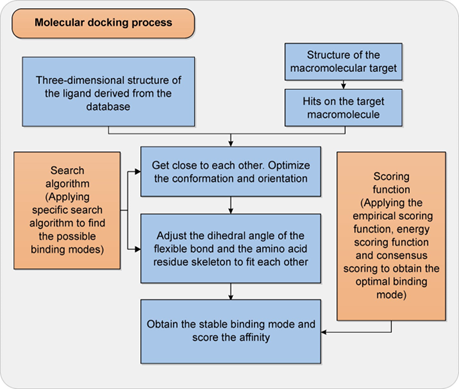
\includegraphics{immagini/processoDockingMolecolare.png}
    \caption{Processo del docking molecolare}
    \label{fig:Processo del docking Molecolare}
\end{figure}

\section{Idea e sviluppo}
L’\textbf{idea} nasce dall’attività di tirocinio svolta presso il "Centro nazionale di ricerca" di Napoli, per un totale di 300 ore (12 CFU), sotto la supervisione del Responsabile del laboratorio professore Angelo Ciaramella e del dottore Ferdinando Febbraio del CNR di Napoli. Il lavoro effettuato è consistito nella realizzazione di un software, del tutto preliminare al progetto di tesi proposto. Lo \textbf{sviluppo} è avvenuto attraverso diverse fasi nelle quali sono stati utilizzati ed implementati i seguenti tools: 

\begin{itemize}
    \item software per l'esecuzione del docking
    \item funzioni di bioinformatica per la preparazione degli input necessari
    \item software per l'analisi dei risultati dell'intero processo.
\end{itemize}

Sono state determinate le componenti software ideali per automatizzare il processo di docking conseguendo risultati efficienti per quanto riguarda l'output e l'analisi dello stesso, offrendo una buona usabilità del prodotto realizzato mediante una semplice ed intuitiva interfaccia grafica.

\section{Contenuto della tesi}
La tesi è divisa in tre moduli:

\begin{itemize}
    \item nella prima parte verranno discusse le tecnologie, le piattaforme scelte per la realizzazione del software, i linguaggi di programmazione e gli strumenti di bioinformatica utilizzati
    \item nella seconda verrà illustrata l'applicazione realizzata, dalla preparazione dei ligandi e recettori, passando per il docking, finendo con l'estrazione dei legami dall'output ottenuto
    \item nell'ultima parte verranno tratte le conclusioni e saranno indicati gli sviluppi futuri del software realizzato.
\end{itemize} 